
\documentclass{article}
\usepackage{tikz}
\usetikzlibrary{shapes.geometric, arrows}


\tikzstyle{start} = [circle, draw=black, fill=white]

\tikzstyle{plani} = [rectangle, rounded corners, minimum width=2cm, minimum height=2cm,text  centered, draw=black, fill=red!30]
\tikzstyle{inv} = [rectangle, rounded corners, minimum width=2cm, minimum height=2cm,text  centered, draw=black, fill=cyan]
\tikzstyle{bkend} = [rectangle, rounded corners, minimum width=2cm, minimum height=2cm,text  centered, draw=black, fill=green]
\tikzstyle{fend} = [rectangle, rounded corners, minimum width=2cm, minimum height=2cm,text  centered, draw=black, fill=gray]

\tikzstyle{io} = [trapezium, trapezium left angle=70, trapezium right angle=110, minimum width=3cm, minimum height=1cm, text centered, draw=black, fill=blue!30]

\tikzstyle{process} = [rectangle, minimum width=3cm, minimum height=1cm, text centered, draw=black, fill=orange!30]

\tikzstyle{decision} = [diamond, minimum width=3cm, minimum height=1cm, text centered, draw=black, fill=green!30]

\tikzstyle{2} = [ultra thick,->,>=stealth,color=red] %Linea gruesa roja
\tikzstyle{1} = [thick,<->,>=stealth, color=black]

\begin{document}

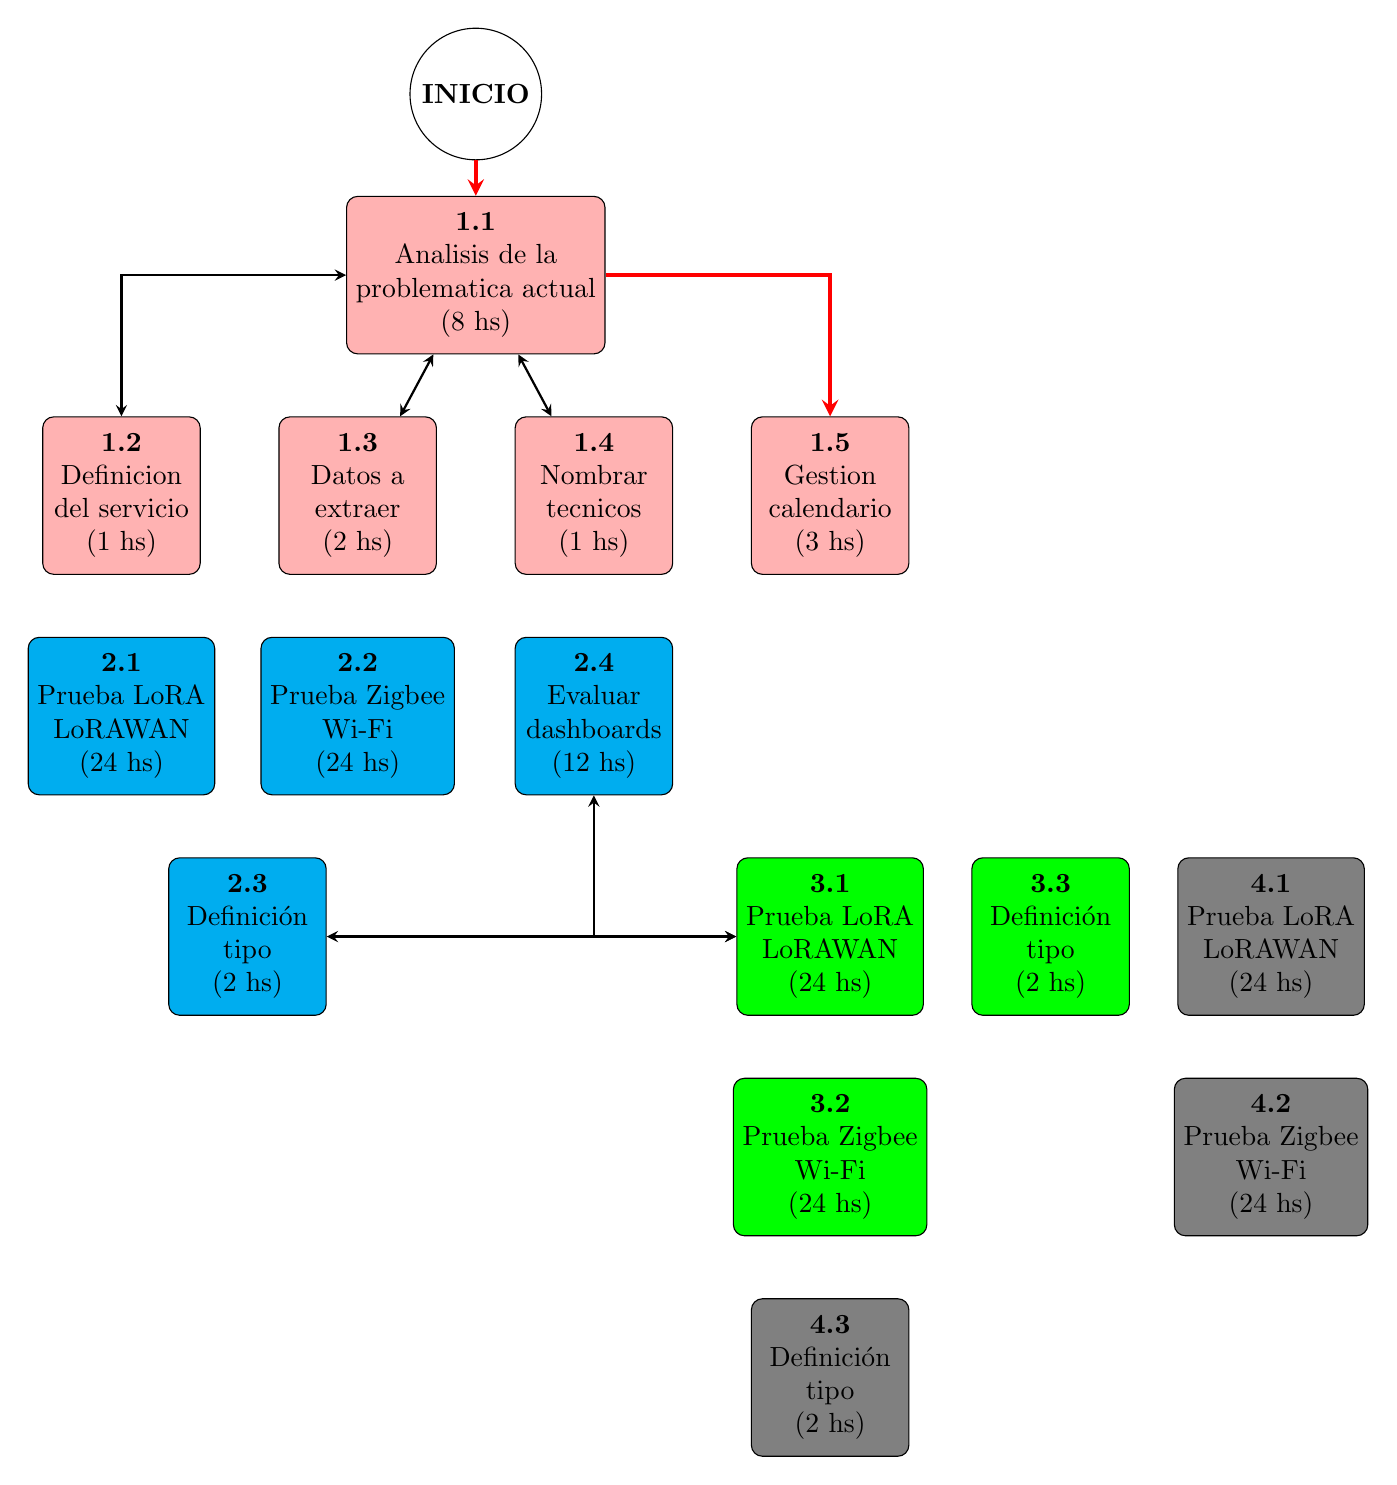
\begin{tikzpicture}[node distance=2cm]
<TikZ code>


\node (inicio) [start, xshift=-2cm] {\textbf {INICIO}};
\node (1_1) [plani, align=flush center, below of=inicio, yshift=-0.3cm] {\textbf{1.1}\\Analisis de la\\ problematica actual\\(8 hs)};
\node (1_2) [plani, align=flush center, below of=1_1,yshift=-0.8cm, xshift=-4.5cm] {\textbf{1.2 }\\Definicion\\del servicio\\(1 hs)};
\node (1_3) [plani, align=flush center, below of=1_1,yshift=-0.8cm, xshift=-1.5cm] {\textbf{1.3}\\Datos a\\ extraer\\(2 hs)};
\node (1_4) [plani, align=flush center, below of=1_1,yshift=-0.8cm, xshift=1.5cm] {\textbf{1.4}\\Nombrar\\ tecnicos\\(1 hs)};
\node (1_5) [plani, align=flush center, below of=1_1,yshift=-0.8cm, xshift=4.5cm] {\textbf{1.5}\\Gestion\\ calendario\\(3 hs)};

\node (2_1) [inv, align=flush center, below of=1_2, yshift=-0.8cm] {\textbf{2.1}\\Prueba LoRA\\ LoRAWAN\\(24 hs)};
\node (2_2) [inv, align=flush center, below of=1_3,yshift=-0.8cm, xshift=0cm] {\textbf{2.2 }\\Prueba Zigbee\\ Wi-Fi\\(24 hs)};
\node (2_3) [inv, align=flush center, below of=2_1,yshift=-0.8cm, xshift=1.6cm] {\textbf{2.3}\\Definición\\ tipo\\(2 hs)};
\node (2_4) [inv, align=flush center, below of=1_4,yshift=-0.8cm, xshift=0cm] {\textbf{2.4}\\Evaluar\\ dashboards\\(12 hs)};

\node (3_1) [bkend, align=flush center, below of=2_4,yshift=-0.8cm, xshift=3cm] {\textbf{3.1}\\Prueba LoRA\\ LoRAWAN\\(24 hs)};
\node (3_2) [bkend, align=flush center, below of=3_1,yshift=-0.8cm, xshift=0cm] {\textbf{3.2 }\\Prueba Zigbee\\ Wi-Fi\\(24 hs)};
\node (3_3) [bkend, align=flush center, right of=3_1, yshift=0cm, xshift=0.8cm] {\textbf{3.3}\\Definición\\ tipo\\(2 hs)};

\node (4_1) [fend, align=flush center, right of=3_3, yshift=0cm, xshift=0.8cm] {\textbf{4.1}\\Prueba LoRA\\ LoRAWAN\\(24 hs)};
\node (4_2) [fend, align=flush center, below of=4_1,yshift=-0.8cm, xshift=0cm] {\textbf{4.2 }\\Prueba Zigbee\\ Wi-Fi\\(24 hs)};
\node (4_3) [fend, align=flush center, below of=3_2,yshift=-0.8cm, xshift=0cm] {\textbf{4.3}\\Definición\\ tipo\\(2 hs)};


\draw [2] (inicio) -- (1_1);
\draw [1] (1_1) -| (1_2);
\draw [1] (1_1) -- (1_3);
\draw [1] (1_1) -- (1_4);
\draw [2] (1_1) -| (1_5);

\draw [1] (2_3) -- (3_1);
\draw [1] (2_4) |- (3_1);


\end{tikzpicture}

\end{document}
